\documentclass[xetex,mathserif,serif]{beamer}
\usepackage{polyglossia}
\setdefaultlanguage[babelshorthands=true]{russian}
\usepackage{minted}
\usepackage{tabu}
\usepackage{pgfplots}
\usepackage{textpos}
\usepackage{subcaption}
\usepackage{graphicx}
\usepackage[normalem]{ulem}

\useoutertheme{infolines}

\usepackage{fontspec}
\setmainfont{FreeSans}
\newfontfamily{\russianfonttt}{FreeSans}

\usepackage{forest}
\usetikzlibrary{arrows}

\setbeamertemplate{blocks}[rounded][shadow=false]
\setbeamercolor*{block title example}{fg=green!50!black,bg=green!20}
\setbeamercolor*{block body example}{fg=black,bg=green!10}

\setbeamercolor*{block title alerted}{fg=red!50!black,bg=red!20}
\setbeamercolor*{block body alerted}{fg=black,bg=red!10}

\newcommand{\attribution}[1] {
	\vspace{-5mm}\begin{flushright}\begin{scriptsize}\textcolor{gray}{\textcopyright\, #1}\end{scriptsize}\end{flushright}
}

\tabulinesep=0.7mm

\title{Хеш-таблицы}
\author[Юрий Литвинов]{Юрий Литвинов \newline \textcolor{gray}{\small\texttt{yurii.litvinov@gmail.com}}}

\date{16.11.2018}

\begin{document}
	
	\frame{\titlepage}

	\begin{frame}
		\frametitle{Хеш-таблица}
		\begin{itemize}
			\item Ещё одна реализация АТД ``множество'' или ``ассоциативный массив''
			\item Требует в среднем константного времени для операций вставки, удаления и поиска
			\begin{itemize}
				\item Быстрее любых деревьев
				\item Очень похожа на массив
			\end{itemize}
			\item Хранит значения неупорядоченными
			\item Сильно зависит от качества хеш-функции
		\end{itemize}
	\end{frame}

	\begin{frame}
		\frametitle{Хеш-функция}
		\begin{columns}
			\begin{column}{0.75\textwidth}
				\begin{itemize}
					\item Некоторая функция, отображающая большое (потенциально бесконечное) множество ключей в конечное (и маленькое) множество хеш-значений
					\begin{itemize}
						\item Не инъективна
					\end{itemize}
					\item Чем ``случайнее'' она это делает, тем лучше
					\begin{itemize}
						\item Немного разным ключам должны соответствовать сильно разные значения
					\end{itemize}
				\end{itemize}
			\end{column}
			\begin{column}{0.25\textwidth}
				\begin{center}
					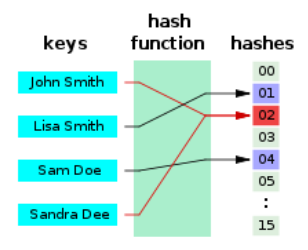
\includegraphics[width=0.95\textwidth]{hashfunction.png}
				\end{center}
			\end{column}
		\end{columns}
		\begin{itemize}
			\item Зачем
			\begin{itemize}
				\item Факторизуем множество ключей по классам эквивалентности, образованным ключами с равными хеш-значениями, будем хранить в массиве фактор-множества\^{}U
				\item Хеш-значения можно использовать как индексы массива, где лежит что-то, что позволяет найти ключ (сегменты), и чем лучше хеш-функция перемешает ключи, тем меньше вероятность коллизии
			\end{itemize}
		\end{itemize}
	\end{frame}

	\begin{frame}
		\frametitle{Хеш-таблица со списками значений}
		\begin{columns}
			\begin{column}{0.5\textwidth}
				\begin{itemize}
					\item Парадокс дней рождения:
					В группе, состоящей из 23 или более человек, вероятность совпадения дней рождения (число и месяц) хотя бы у двух людей превышает 50\%
					\item Будем хранить в массиве список ключей с одинаковым хеш-значением
					\begin{itemize}
						\item Можно и самобалансирующееся двоичное дерево поиска, чтобы быстро найти нужный ключ
						\begin{itemize}
							\item Но не нужно
						\end{itemize}
					\end{itemize}
				\end{itemize}
			\end{column}
			\begin{column}{0.5\textwidth}
				\begin{center}
					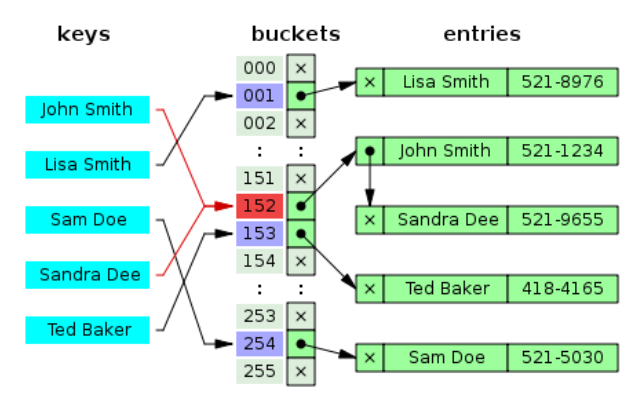
\includegraphics[width=0.9\textwidth]{hashtable.png}
				\end{center}
			\end{column}
		\end{columns}
	\end{frame}

	\begin{frame}
		\frametitle{Хеш-таблица, ``открытая адресация''}
		\begin{columns}
			\begin{column}{0.55\textwidth}
				\begin{itemize}
					\item Второй способ: будем хранить в хеш-таблице сами ключи со значениями, а если ячейка уже занята, брать следующую (может быть, по какому-нибудь сложному правилу)
					\item Удаление требует дополнительной информации
					\begin{itemize}
						\item Пустая ячейка будет воспринята как конец цепочки
						\item Обычно делают флаг ``ячейка была удалена''
						\begin{itemize}
							\item При вставке --- вставляют
							\item При поиске и удалении --- идут дальше
						\end{itemize}
					\end{itemize}
				\end{itemize}
			\end{column}
			\begin{column}{0.45\textwidth}
				\begin{center}
					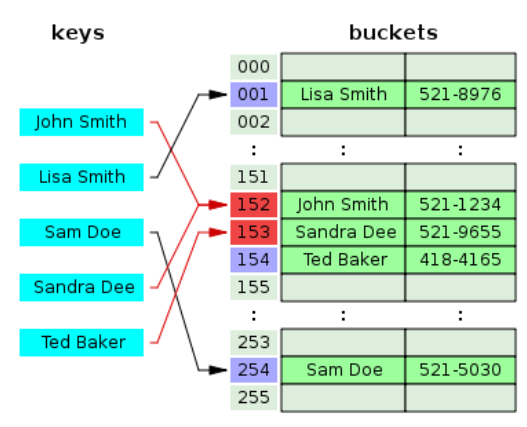
\includegraphics[width=0.9\textwidth]{hashtable-with-open-addressing.png}
				\end{center}
			\end{column}
		\end{columns}
	\end{frame}

	\begin{frame}
		\frametitle{Коэффициент заполнения}
		Пусть $n$ --- число элементов в хеш-таблице, $k$ --- число сегментов (в английской литературе сегменты называются buckets). Коэффициент заполнения хеш-таблицы $L = n / k$
		\begin{columns}
			\begin{column}{0.5\textwidth}
				\begin{itemize}
					\item Коэффициент заполнения должен быть примерно равен $1$ для хеш-таблиц со списками и $< 0.7$ для хеш-таблиц с открытой адресацией
					\begin{itemize}
						\item Динамическое изменение размеров массива
						\begin{itemize}
							\item Требуется заново переложить все значения
						\end{itemize}
					\end{itemize}
				\end{itemize}
			\end{column}
			\begin{column}{0.5\textwidth}
				\begin{center}
					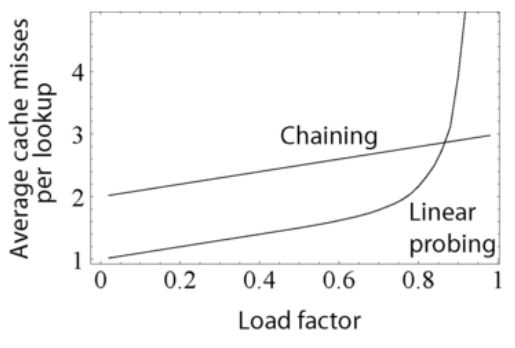
\includegraphics[width=0.9\textwidth]{load-factor.png}
				\end{center}
			\end{column}
		\end{columns}
	\end{frame}

	\begin{frame}[fragile]
		\frametitle{Выбор хеш-функции}
		\begin{itemize}
			\item Должна быть возможно более случайной
			\item Должна зависеть только от ключа
			\item Должна считаться быстро
			\item Например:
			\begin{footnotesize}
				\begin{minted}{cpp}
int h(char *value) {
    int result = 0;
    for (int i = 0; value[i] != '\0'; ++i)
        result = (result + value[i]) % hashSize;
    return result;
}
				\end{minted}
			\end{footnotesize}
			\item Обычно хеш-функция возвращает просто целое число, а хеш-таблица сама ``загоняет'' его в нужный диапазон значений
		\end{itemize}
	\end{frame}

	\begin{frame}
		\frametitle{Ещё про хеш-функции}
		\begin{itemize}
			\item Для целых чисел вполне сойдёт id
			\item ``Совершенная хеш-функция'' --- инъективна
			\item Универсальная хеш-функция --- семейство функций
			\item Криптографические хеш-функции
			\begin{itemize}
				\item MD5
				\item SHA1
				\item Небыстро считаются, поэтому не подходят
			\end{itemize}
			\item Хеш-функции для сложных типов данных
			\begin{itemize}
				\item Сумма или произведение хеш-функций элементов, как для строки
				\begin{itemize}
					\item Значение полинома $a[0]*p^n + a[1]*p^{n - 1} + … + a[n]$, особенно если $p$ --- простое (Rolling hash)
				\end{itemize}
				\item xor хеш-функций элементов
			\end{itemize}
		\end{itemize}
	\end{frame}

\end{document}